%% Default preamble BEGIN
\documentclass[oneside]{memoir}

\usepackage{./documenter}
\usepackage{./custom}

%% Title Page
\title{
    {\HUGE \DocMainTitle }\\
    {\Large \DocVersion }
}
\author{ \DocAuthors }

%% TOC settings
% -- TOC depth
%   value: [part, chapter, section, subsection,
%           subsubsection, paragraph, subparagraph]
\settocdepth{section}  % show "part+chapter+section" in TOC
% -- TOC spacing
%   ref: https://tex.stackexchange.com/questions/60317/toc-spacing-in-memoir
%   doc: memoir/memman.pdf
%       - Figure 9.2: Layout of a ToC
%       - Table 9.3: Value of K in macros for styling entries
\makeatletter
% {part} to {chapter}
\setlength{\cftbeforepartskip}{1.5em \@plus \p@}
% {chapter} to {chapter}
\setlength{\cftbeforechapterskip}{0.0em \@plus \p@}
% Chapter num to chapter title spacing (Figure 9.2@memman)
\setlength{\cftchapternumwidth}{2.5em \@plus \p@}
% indent before section number
\setlength{\cftsectionindent}{2.5em \@plus \p@}
% Section num to section title spacing (Figure 9.2@memman)
\setlength{\cftsectionnumwidth}{4.0em \@plus \p@}
\makeatother

%% Main document begin
\begin{document}

\frontmatter
\maketitle
\clearpage
\tableofcontents

\mainmatter
%% preamble END

% Useful variables
\newcommand{\DocMainTitle}{Juscan.jl}
\newcommand{\DocVersion}{}
\newcommand{\DocAuthors}{lihuax(LiZehua)}
\newcommand{\JuliaVersion}{1.11.3}

% ---- Insert preamble
% \input{preamble.tex}


\part{Home}


Juscan.jl is a Julia implementation of Scanpy, tailored for single-cell data analysis. Currently in its development (dev) version, the library aims to deliver high-performance, flexible, and extensible tools for preprocessing, dimensionality reduction, clustering, and visualization of single-cell datasets.



\section{Features}



\label{7269310191258299096}{}


\begin{itemize}
\item \textbf{Single-Cell Data Analysis}   Provides functionalities for data normalization, log transformation, dimensionality reduction (e.g., PCA), and graph-based clustering (e.g., Leiden algorithm).


\item \textbf{High Performance Computing}   Leverages Julia{\textquotesingle}s computational strengths to efficiently handle large-scale single-cell datasets.


\item \textbf{Modular and Extensible}   Designed with a modular architecture, allowing users to easily customize and extend functionality to suit diverse analytical requirements.

\end{itemize}


\section{Development Status}



\label{17041994431004078622}{}


Juscan.jl is under active development. Some features are still being refined and may change over time. We welcome feedback, bug reports, and contributions from the community.



\section{Installation}



\label{16848947351613073531}{}


\subsection{Installing the Development Version via Julia Package Manager}



\label{5101380886399676247}{}


You can install the development version using Julia{\textquotesingle}s package manager:




\begin{minted}{julia}
using Pkg
Pkg.add(url="https://github.com/zehua0417/Juscan.jl")
\end{minted}



\subsection{Cloning the Repository for Local Development}



\label{10997474127977679411}{}



\begin{minted}{text}
git clone https://github.com/zehua0417/Juscan.jl.git
cd Juscan.jl
julia --project -e 'using Pkg; Pkg.instantiate()'
\end{minted}



\section{Quick Start Example}



\label{1185376811553284019}{}


Here’s a simple example demonstrating basic single-cell data preprocessing and analysis with Juscan.jl:




\begin{minted}{julia}
using Juscan

# Load the dataset
adata = Juscan.readh5ad("data/data.h5ad")

# Quality control
Juscan.Pp.filter_cells!(adata, min_genes=100, max_genes=8000, max_counts=140000)
Juscan.Pp.filter_genes!(adata, min_cells=3)
adata.var.mt = startswith.(adata.var_names, "MT-")
Juscan.Pp.calculate_qc_metrics!(adata, qc_vars=["mt"])

# Normalization and log transformation
adata.layers["normalized"] = deepcopy(adata.X)
Juscan.Pp.normalize_total!(adata, target_sum=1000, layer="normalized")
Juscan.Tl.logp1_transform!(adata, layer="normalized", key_added="normalized_logp1")

# Highly variable genes and PCA
Juscan.Tl.highly_variable_genes!(adata, n_top_genes=2000, layer="normalized_logp1")
Juscan.Tl.pca!(adata; layer="normalized_logp1", key_added="pca", n_pcs=15)

# Clustering and UMAP visualization
Juscan.Tl.clustering!(adata, method="km", use_pca=15, cluster_K=4)
Juscan.Tl.umap!(adata; key_added="umap", n_pcs=15, use_pca="pca")
Juscan.Pl.plot_umap(adata, color_by="clusters_0.5")
\end{minted}



\section{Contributing}



\label{2097515079362899065}{}


We welcome contributions of all kinds:



\begin{itemize}
\item \textbf{Bug Reports \& Suggestions}: Please open an issue on GitHub.


\item \textbf{Code or Documentation Updates}.


\item \textbf{Discussions}: Share your feedback and experiences to help improve the project.

\end{itemize}


\section{License}



\label{2455754727547577773}{}


Juscan.jl is licensed under the MIT License.



\section{Contact}



\label{15110382712247013745}{}


If you have any questions or suggestions, please open an issue on GitHub or contact us at \href{mailto:zehuali0417@gmail.com}{my e-mail}.



\section{Acknowledgments}



\label{6467028106495259876}{}


We would like to extend our sincere gratitude to the open source community for their continuous support and inspiration. In particular, we thank:



\begin{itemize}
\item \href{https://github.com/theislab/scanpy}{Scanpy} for its groundbreaking approach to single-cell analysis,


\item \href{https://github.com/theislab/anndata}{AnnData} for providing a robust data structure for annotated data,


\item \href{https://github.com/scverse/Muon.jl.git}{Muon.jl} for its innovative multi-omic analysis tools, and


\item \href{https://github.com/kaji331/ASCT}{Automatic Single-cell Toolbox (ASCT)}:An automated single-cell data analysis toolbox inspired by Seurat v4 in R.


\item \href{https://github.com/maren-ha/scVI.jl.git}{scVI.jl} for offering valuable insights into variational inference methods.

\end{itemize}


Their contributions and ideas have been instrumental in shaping the development and direction of Juscan.jl.



{\rule{\textwidth}{1pt}}


Thank you for your interest in Juscan.jl. We hope it will empower your single-cell data analysis projects!



\part{Tutorial}


\chapter{Quick Start}


\section{Quick Start Guide for Juscan.jl}



\label{12683719284981916232}{}


This guide walks you through a basic single-cell RNA-seq analysis pipeline using \href{https://github.com/zehua0417/Juscan.jl}{\texttt{Juscan.jl}}. The dataset used in this example comes from \href{https://doi.org/10.6084/m9.figshare.22716739.v1}{doi:10.6084/m9.figshare.22716739.v1}.



\subsection{📦 Prerequisites}



\label{15702409122439959613}{}


Make sure you have installed \texttt{Juscan.jl}, \texttt{Muon.jl}, and their dependencies:




\begin{minted}{julia}
using Pkg
Pkg.activate(".")
Pkg.add(url="https://github.com/zehua0417/Juscan.jl")
\end{minted}



\subsection{📁 Load Data}



\label{2195623716691941297}{}



\begin{minted}{julia}
using Juscan
using Muon
using DataFrames

adata = Juscan.readh5ad("data/data.h5ad")
\end{minted}



\subsection{🔍 Quality Control}



\label{5697303154653018679}{}



\begin{minted}{julia}
Juscan.Pp.filter_cells!(adata, min_genes=100)
Juscan.Pp.filter_genes!(adata, min_cells=3)
Juscan.Pp.filter_cells!(adata, max_genes=8000)
Juscan.Pp.filter_cells!(adata, max_counts=140000)

adata.var.mt = startswith.(adata.var_names, "MT-")
adata.var.ribo = startswith.(adata.var_names, "RPS") .| startswith.(adata.var_names, "RPL")
adata.var.hb = occursin.(r"^HB[^P]", adata.var_names)

Juscan.Pp.calculate_qc_metrics!(adata, qc_vars=["mt", "ribo", "hb"])
\end{minted}



\subsubsection{📊 Visualize QC Metrics}



\label{18287271198092503872}{}



\begin{minted}{julia}
Juscan.Pl.violin(
  adata,
  ["pct_counts_mt", "n_genes_by_counts", "total_counts"];
  width=300,
  height=800,
  fill_alpha=0.7,
  savefig="/home/lihuax/Pictures/Juscan/qc_violin.png",
)

Juscan.Pl.scatter(
  adata,
  "total_counts",
  "n_genes_by_counts",
  color_key="pct_counts_mt",
  width=800,
  height=800,
  colormap_name="magma",
  savefig="/home/lihuax/Pictures/Juscan/qc_scatter.png",
)
\end{minted}



\subsection{🔬 Normalization}



\label{12632274355541218568}{}



\begin{minted}{julia}
adata.layers["normalized"] = deepcopy(adata.X)
Juscan.Pp.normalize_total!(adata, target_sum=1000, layer="normalized")
Juscan.Tl.logp1_transform!(adata, layer="normalized", key_added="normalized_logp1")
adata.layers["normalized_logp1"] = Float64.(adata.layers["normalized_logp1"])
\end{minted}



\subsection{🧬 Highly Variable Genes}



\label{4519193584898427520}{}



\begin{minted}{julia}
Juscan.Tl.highly_variable_genes!(adata, n_top_genes=2000, layer="normalized_logp1")
Juscan.Pl.hvg_scatter(adata, savefig="/home/lihuax/Pictures/Juscan/hvg_scatter.png")
\end{minted}



\subsection{📉 Dimensionality Reduction}



\label{11472669785569077732}{}



\begin{minted}{julia}
Juscan.Tl.pca!(adata; key_added="pca", n_pcs=15)
Juscan.Tl.pca!(adata; layer="normalized_logp1", key_added="pca", n_pcs=15)
Juscan.Pl.plot_variance_ratio(adata, savefig="/home/lihuax/Pictures/Juscan/variance_ratio.png")

Juscan.Tl.subset_to_hvg!(adata; layer="normalized_logp1", n_top_genes=2000)
Juscan.Pp.filter_cells!(adata, min_counts=3000)
Juscan.Pp.filter_cells!(adata, max_counts=10000)
\end{minted}



\subsection{🔗 Clustering \& UMAP}



\label{4391682998113665460}{}



\begin{minted}{julia}
Juscan.Tl.clustering!(adata, method="km", use_pca=15, cluster_K=4, dist="Euclidean")
Juscan.Tl.umap!(
  adata;
  key_added="umap",
  use_pca="pca",
  n_pcs=15,
  min_dist=0.5,
  n_neighbors=50,
)
fig = Juscan.Pl.plot_umap(adata, color_by="clusters_0.5")
\end{minted}



{\rule{\textwidth}{1pt}}


This pipeline demonstrates the essential steps of scRNA-seq analysis using \texttt{Juscan.jl}. For more detailed usage, please refer to the \href{https://zehua0417.github.io/Juscan.jl/}{official documentation}.



Happy analyzing! 🧬✨



\part{API}


\chapter{Anndata Utils}


\section{AnnData Module}



\label{4706097015300978284}{}


The \texttt{AnnData} struct is imported from \href{https://github.com/scverse/Muon.jl}{\texttt{Muon.jl}}. The package provides read and write functions for \texttt{.h5ad} and \texttt{.h5mu} files, the typical H5-based format for storing Python \texttt{anndata} objects. The \texttt{AnnData} object stores datasets together with metadata, such as information on the variables (genes in scRNA-seq data) and observations (cells), as well as different kinds of annotations and transformations of the original count matrix, such as PCA or UMAP embeddings, or graphs of observations or variables.



For details on the Julia implementation in \texttt{Muon.jl}, see the \href{https://scverse.github.io/Muon.jl/dev/}{documentation}.



For more details on the original Python implementation of the \texttt{anndata} object, see the \href{https://anndata.readthedocs.io/en/latest/}{documentation} and \href{https://doi.org/10.1101/2021.12.16.473007}{preprint}.



\begin{figure}
\centering
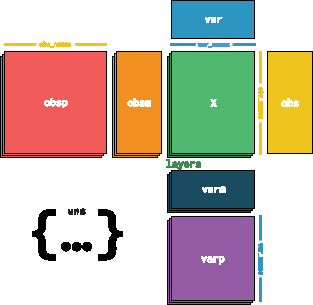
\includegraphics[max width=\linewidth]{assets/anndata_schema.png}
\caption{anndata}
\end{figure}



\begin{itemize}
\item \hyperlinkref{2502770603687263729}{\texttt{Juscan.get\_celltypes}}
\item \hyperlinkref{824771256157212624}{\texttt{Juscan.insert\_obs!}}
\item \hyperlinkref{4357925709652045163}{\texttt{Juscan.insert\_var!}}
\item \hyperlinkref{11445546764670757650}{\texttt{Juscan.subset\_adata}}
\item \hyperlinkref{2261814719333819436}{\texttt{Juscan.subset\_adata!}}
\end{itemize}


\subsection{celltypes}



\label{5500776454038897893}{}

\hypertarget{2502770603687263729}{\texttt{Juscan.get\_celltypes}}  -- {Function.}

\begin{adjustwidth}{2em}{0pt}


\begin{minted}{julia}
get_celltypes(a::AnnData)
\end{minted}

Tries to infer the cell types of cells in an \texttt{AnnData} object. 

Returns a vector of cell type names if the cell types are stored in  \texttt{adata.obs[{\textquotedbl}cell\_type{\textquotedbl}]}, \texttt{adata.obs[{\textquotedbl}celltype{\textquotedbl}]}, \texttt{adata.obs[{\textquotedbl}celltypes{\textquotedbl}]}, or \texttt{adata.obs[{\textquotedbl}cell\_types{\textquotedbl}]}.  Otherwise, returns \texttt{nothing}.



\href{https://github.com/zehua0417/Juscan.jl/blob/393ad1b827b678ea98a738f92af658ee9ed9a403/src/anndata.jl#L46-L54}{\texttt{source}}


\end{adjustwidth}

\subsection{subset adata}



\label{17184326838247328209}{}

\hypertarget{11445546764670757650}{\texttt{Juscan.subset\_adata}}  -- {Function.}

\begin{adjustwidth}{2em}{0pt}


\begin{minted}{julia}
subset_adata(adata::AnnData, subset_inds::Tuple, dims::Symbol=:both)
\end{minted}

Subset an \texttt{AnnData} object by indices passed as a tuple of vectors of integers, UnitRanges, or vectors of Booleans. If \texttt{dims} is set to :both, the first element of \texttt{subset\_inds} is used to subset cells and the second element is used to subset genes.

\textbf{Arguments}

\begin{itemize}
\item \texttt{adata}: \texttt{AnnData} object to subset


\item \texttt{subset\_inds}: tuple of vectors of integers, UnitRanges, or vectors of Booleans


\item \texttt{dims}: dimension to subset, either \texttt{:cells}, \texttt{:genes}, or \texttt{:both}

\end{itemize}
\textbf{Returns}

\begin{itemize}
\item a copy of the \texttt{AnnData} object with the subsetted data

\end{itemize}


\href{https://github.com/zehua0417/Juscan.jl/blob/393ad1b827b678ea98a738f92af658ee9ed9a403/src/anndata.jl#L195-L208}{\texttt{source}}



\begin{minted}{julia}
subset_adata(adata::AnnData, subset_inds::Union{Int, Vector{Int}, UnitRange, Vector{Bool}}, dims::Symbol)
\end{minted}

Subset an \texttt{AnnData} object by indices passed as a vector of integers or booleans or as a UnitRange.  The \texttt{dims} argument can be set to either \texttt{:cells} or \texttt{:genes} to specify which dimension to subset. 

\textbf{Arguments}

\begin{itemize}
\item \texttt{adata}: \texttt{AnnData} object to subset


\item \texttt{subset\_inds}: vector of integers or booleans or UnitRange


\item \texttt{dims}: dimension to subset, either \texttt{:cells} or \texttt{:genes}

\end{itemize}
\textbf{Returns}

\begin{itemize}
\item a copy of the \texttt{AnnData} object with the subsetted data

\end{itemize}


\href{https://github.com/zehua0417/Juscan.jl/blob/393ad1b827b678ea98a738f92af658ee9ed9a403/src/anndata.jl#L215-L228}{\texttt{source}}


\end{adjustwidth}
\hypertarget{2261814719333819436}{\texttt{Juscan.subset\_adata!}}  -- {Function.}

\begin{adjustwidth}{2em}{0pt}


\begin{minted}{julia}
subset_adata!(adata::AnnData, subset_inds, dims::Symbol)
\end{minted}

In-place version of \texttt{subset\_adata}, see \texttt{?subset\_adata} for more details. 

For \texttt{subset\_inds}, either a tuple of vectors or ranges can be passed with \texttt{dims} set to :both, for subsetting  both cells and genes, or a single vector or range can be passed with \texttt{dims} set to either :cells or :genes.

\textbf{Arguments}

\begin{itemize}
\item \texttt{adata}: \texttt{AnnData} object to subset


\item \texttt{subset\_inds}: tuple of vectors of integers, UnitRanges, or vectors of Booleans or vector of integers or booleans or UnitRange


\item \texttt{dims}: dimension to subset, either \texttt{:cells}, \texttt{:genes}, or \texttt{:both}

\end{itemize}
\textbf{Returns}

\begin{itemize}
\item the \texttt{AnnData} object with the subsetted data

\end{itemize}


\href{https://github.com/zehua0417/Juscan.jl/blob/393ad1b827b678ea98a738f92af658ee9ed9a403/src/anndata.jl#L239-L254}{\texttt{source}}


\end{adjustwidth}

\subsection{insert}



\label{5057365744536548781}{}

\hypertarget{824771256157212624}{\texttt{Juscan.insert\_obs!}}  -- {Function.}

\begin{adjustwidth}{2em}{0pt}


\begin{minted}{julia}
insert_obs!(adata::AnnData, obs::DataFrame)
\end{minted}

Insert new columns into the \texttt{obs} DataFrame of an \texttt{AnnData} object.

\textbf{Arguments}

\begin{itemize}
\item \texttt{adata}: The \texttt{AnnData} object to modify.


\item \texttt{obs}: A DataFrame containing the new columns to be inserted. The number of rows in \texttt{obs} must match the number of cells in \texttt{adata}.

\end{itemize}
\textbf{Returns}

\begin{itemize}
\item \texttt{nothing}: Modifies the \texttt{adata.obs} DataFrame in place.

\end{itemize}
\textbf{Notes}

\begin{itemize}
\item This function assumes that the number of rows in \texttt{obs} matches the number of cells in \texttt{adata}. If they do not match, an error will be thrown.


\item This function modifies the \texttt{adata.obs} DataFrame directly. If you want to keep the original \texttt{adata} unchanged, make a copy before calling this function.

\end{itemize}


\href{https://github.com/zehua0417/Juscan.jl/blob/393ad1b827b678ea98a738f92af658ee9ed9a403/src/anndata.jl#L359-L374}{\texttt{source}}


\end{adjustwidth}
\hypertarget{4357925709652045163}{\texttt{Juscan.insert\_var!}}  -- {Function.}

\begin{adjustwidth}{2em}{0pt}


\begin{minted}{julia}
insert_var!(adata::AnnData, var::DataFrame)
\end{minted}

Insert new columns into the \texttt{var} DataFrame of an \texttt{AnnData} object.

\textbf{Arguments}

\begin{itemize}
\item \texttt{adata}: The \texttt{AnnData} object to modify.


\item \texttt{var}: A DataFrame containing the new columns to be inserted. The number of rows in \texttt{var} must match the number of genes in \texttt{adata}.

\end{itemize}
\textbf{Returns}

\begin{itemize}
\item \texttt{nothing}: Modifies the \texttt{adata.var} DataFrame in place.

\end{itemize}
\textbf{Notes}

\begin{itemize}
\item This function assumes that the number of rows in \texttt{var} matches the number of genes in \texttt{adata}. If they do not match, an error will be thrown.


\item This function modifies the \texttt{adata.var} DataFrame directly. If you want to keep the original \texttt{adata} unchanged, make a copy before calling this function.

\end{itemize}


\href{https://github.com/zehua0417/Juscan.jl/blob/393ad1b827b678ea98a738f92af658ee9ed9a403/src/anndata.jl#L381-L396}{\texttt{source}}


\end{adjustwidth}

\chapter{Preprocessing}


\section{Preprocessing Module}



\label{7637094317854373936}{}


Preprocessing is a crucial step in single-cell and multi-omics data analysis. This module provides functions for quality control, filtering, and normalization to ensure that datasets are clean and ready for downstream analyses.



Quality control (QC) metrics help identify low-quality cells and genes, such as those with extremely high or low counts, high dropout rates, or disproportionate expression levels. By computing these metrics, users can apply appropriate thresholds to retain only reliable data.



Filtering enables users to remove unwanted cells or genes based on QC criteria, ensuring that low-quality features do not affect downstream analyses.



Normalization methods adjust for differences in sequencing depth and technical variation, allowing meaningful comparisons across cells and conditions.



These preprocessing functions ensure that data is well-structured and suitable for clustering, dimensionality reduction, and other analytical tasks.


\begin{itemize}
\item \hyperlinkref{16333846089314708702}{\texttt{Juscan.Pp.calculate\_qc\_metrics}}
\item \hyperlinkref{4940879531160147877}{\texttt{Juscan.Pp.calculate\_qc\_metrics!}}
\item \hyperlinkref{18028582656875801779}{\texttt{Juscan.Pp.describe\_obs}}
\item \hyperlinkref{4701942048935169455}{\texttt{Juscan.Pp.describe\_obs!}}
\item \hyperlinkref{17037237803751367329}{\texttt{Juscan.Pp.describe\_var}}
\item \hyperlinkref{17655604818096302154}{\texttt{Juscan.Pp.describe\_var!}}
\item \hyperlinkref{9396744289236617891}{\texttt{Juscan.Pp.filter\_cells}}
\item \hyperlinkref{1074066941160685150}{\texttt{Juscan.Pp.filter\_cells!}}
\item \hyperlinkref{8931327722432789847}{\texttt{Juscan.Pp.filter\_genes}}
\item \hyperlinkref{9061421341658437259}{\texttt{Juscan.Pp.filter\_genes!}}
\item \hyperlinkref{8549673828608603299}{\texttt{Juscan.Pp.normalize\_total}}
\item \hyperlinkref{13118707542266310213}{\texttt{Juscan.Pp.normalize\_total!}}
\end{itemize}


\subsection{quality control metrics}



\label{12647796871482763015}{}

\hypertarget{16333846089314708702}{\texttt{Juscan.Pp.calculate\_qc\_metrics}}  -- {Function.}

\begin{adjustwidth}{2em}{0pt}


\begin{minted}{julia}
calculate_qc_metrics!(adata; expr_type="counts", var_type="genes", qc_vars=String[], 
                      percent_top=[50, 100, 200, 500], layer=nothing, use_raw=false, 
                      use_log1p=true, parallel=nothing) -> Tuple{DataFrame, DataFrame}
\end{minted}

Calculate quality control metrics and return.

\textbf{Arguments}

\begin{itemize}
\item \texttt{adata}: \texttt{Muon.AnnData}   Annotated data matrix containing single-cell or multi-omics data.


\item \texttt{expr\_type}: \texttt{String} (default: \texttt{{\textquotedbl}counts{\textquotedbl}})   The type of expression data to use, such as raw counts or normalized values.


\item \texttt{var\_type}: \texttt{String} (default: \texttt{{\textquotedbl}genes{\textquotedbl}})   Specifies the variable type, e.g., \texttt{{\textquotedbl}genes{\textquotedbl}} for gene expression.


\item \texttt{qc\_vars}: \texttt{Union\{Vector\{String\}, String\}} (default: \texttt{String[]})   A list of quality control variables to consider. If a single string is provided, it will be converted to a vector.


\item \texttt{percent\_top}: \texttt{Union\{Vector\{Int\}, Nothing\}} (default: \texttt{[50, 100, 200, 500]})   A list of top feature (e.g., gene) counts to compute the percentage of total counts for each cell.


\item \texttt{layer}: \texttt{Union\{String, Nothing\}} (default: \texttt{nothing})   Specifies the layer in \texttt{adata} to use. If \texttt{nothing}, the default matrix is used.


\item \texttt{use\_raw}: \texttt{Bool} (default: \texttt{false})   Whether to use the raw counts matrix (\texttt{adata.raw}) instead of the processed data.


\item \texttt{use\_log1p}: \texttt{Bool} (default: \texttt{true})   Whether to apply \texttt{log1p} transformation to the data before computing quality control metrics.


\item \texttt{parallel}: \texttt{Union\{Bool, Nothing\}} (default: \texttt{nothing})   \textbf{(Deprecated)} This argument is ignored but retained for backward compatibility.

\end{itemize}
\textbf{Returns}

\begin{itemize}
\item A tuple of two \texttt{DataFrames.DataFrame}:  

\begin{itemize}
\item[1. ] The first \texttt{DataFrame} contains per-cell quality control metrics.  


\item[2. ] The second \texttt{DataFrame} contains per-gene quality control metrics.

\end{itemize}
\end{itemize}


\href{https://github.com/zehua0417/Juscan.jl/blob/393ad1b827b678ea98a738f92af658ee9ed9a403/src/preprocessing/qc.jl#L11-L42}{\texttt{source}}


\end{adjustwidth}
\hypertarget{4940879531160147877}{\texttt{Juscan.Pp.calculate\_qc\_metrics!}}  -- {Function.}

\begin{adjustwidth}{2em}{0pt}


\begin{minted}{julia}
calculate_qc_metrics!(adata; expr_type="counts", var_type="genes", qc_vars=String[], 
                      percent_top=[50, 100, 200, 500], layer=nothing, use_raw=false, 
                      use_log1p=true, parallel=nothing) -> Nothing
\end{minted}

Calculate and store quality control (QC) metrics directly in the \texttt{obs} and \texttt{var} attributes of \texttt{adata}.

\textbf{Arguments}

\begin{itemize}
\item \texttt{adata}: \texttt{Muon.AnnData}   Annotated data matrix containing single-cell or multi-omics data.   The QC metrics will be stored in \texttt{adata.obs} (per-cell) and \texttt{adata.var} (per-gene).


\item \texttt{expr\_type}: \texttt{String} (default: \texttt{{\textquotedbl}counts{\textquotedbl}})   The type of expression data to use, such as raw counts or normalized values.


\item \texttt{var\_type}: \texttt{String} (default: \texttt{{\textquotedbl}genes{\textquotedbl}})   Specifies the variable type, e.g., \texttt{{\textquotedbl}genes{\textquotedbl}} for gene expression.


\item \texttt{qc\_vars}: \texttt{Union\{Vector\{String\}, String\}} (default: \texttt{String[]})   A list of quality control variables to consider. If a single string is provided, it will be converted to a vector.


\item \texttt{percent\_top}: \texttt{Union\{Vector\{Int\}, Nothing\}} (default: \texttt{[50, 100, 200, 500]})   A list of top feature (e.g., gene) counts to compute the percentage of total counts for each cell.


\item \texttt{layer}: \texttt{Union\{String, Nothing\}} (default: \texttt{nothing})   Specifies the layer in \texttt{adata} to use. If \texttt{nothing}, the default matrix is used.


\item \texttt{use\_raw}: \texttt{Bool} (default: \texttt{false})   Whether to use the raw counts matrix (\texttt{adata.raw}) instead of the processed data.


\item \texttt{use\_log1p}: \texttt{Bool} (default: \texttt{true})   Whether to apply \texttt{log1p} transformation to the data before computing quality control metrics.


\item \texttt{parallel}: \texttt{Union\{Bool, Nothing\}} (default: \texttt{nothing})   \textbf{(Deprecated)} This argument is ignored but retained for backward compatibility.

\end{itemize}
\textbf{Returns}

\begin{itemize}
\item \texttt{Nothing}:   This function modifies \texttt{adata} in place by adding QC metrics to \texttt{adata.obs} and \texttt{adata.var}.

\end{itemize}
\textbf{Notes}

\begin{itemize}
\item Unlike \texttt{calculate\_qc\_metrics}, which returns QC metrics as \texttt{DataFrame} objects,   this function directly updates \texttt{adata} without returning any values.

\end{itemize}


\href{https://github.com/zehua0417/Juscan.jl/blob/393ad1b827b678ea98a738f92af658ee9ed9a403/src/preprocessing/qc.jl#L87-L122}{\texttt{source}}


\end{adjustwidth}

\subsubsection{sub functions}



\label{7062540350669265862}{}

\hypertarget{18028582656875801779}{\texttt{Juscan.Pp.describe\_obs}}  -- {Function.}

\begin{adjustwidth}{2em}{0pt}


\begin{minted}{julia}
describe_obs(adata; expr_type="counts", var_type="genes", qc_vars=String[], 
             percent_top=[50, 100, 200, 500], layer=nothing, use_raw=false, 
             use_log1p=true, X=nothing, parallel=nothing) -> DataFrames.DataFrame
\end{minted}

Compute per-cell quality control (QC) metrics from the expression matrix and return them as a \texttt{DataFrame}.

\textbf{Arguments}

\begin{itemize}
\item \texttt{adata}: \texttt{Muon.AnnData}   Annotated data matrix containing single-cell or multi-omics data.


\item \texttt{expr\_type}: \texttt{String} (default: \texttt{{\textquotedbl}counts{\textquotedbl}})   The type of expression data to use, such as raw counts or normalized values.


\item \texttt{var\_type}: \texttt{String} (default: \texttt{{\textquotedbl}genes{\textquotedbl}})   Specifies the variable type, e.g., \texttt{{\textquotedbl}genes{\textquotedbl}} for gene expression.


\item \texttt{qc\_vars}: \texttt{Union\{Vector\{String\}, String\}} (default: \texttt{String[]})   A list of quality control variables to consider. If a single string is provided, it will be converted to a vector.


\item \texttt{percent\_top}: \texttt{Union\{Vector\{Int\}, Nothing\}} (default: \texttt{[50, 100, 200, 500]})   A list of top feature (e.g., gene) counts to compute the percentage of total counts for each cell.


\item \texttt{layer}: \texttt{Union\{String, Nothing\}} (default: \texttt{nothing})   Specifies the layer in \texttt{adata} to use. If \texttt{nothing}, the default matrix is used.


\item \texttt{use\_raw}: \texttt{Bool} (default: \texttt{false})   Whether to use the raw counts matrix (\texttt{adata.raw}) instead of the processed data.


\item \texttt{use\_log1p}: \texttt{Bool} (default: \texttt{true})   Whether to apply \texttt{log1p} transformation to the data before computing quality control metrics.


\item \texttt{X}: \texttt{Union\{Nothing, SparseMatrixCSC\}} (default: \texttt{nothing})   The expression matrix to use. If \texttt{nothing}, the matrix is determined by \texttt{\_choose\_mtx\_rep}.


\item \texttt{parallel}: \texttt{Union\{Bool, Nothing\}} (default: \texttt{nothing})   \textbf{(Deprecated)} This argument is ignored but retained for backward compatibility.

\end{itemize}
\textbf{Returns}

\begin{itemize}
\item \texttt{DataFrames.DataFrame}:   A \texttt{DataFrame} containing per-cell QC metrics, including:

\begin{itemize}
\item \texttt{{\textquotedbl}n\_\$(var\_type)\_by\_\$(expr\_type){\textquotedbl}}: Number of detected features per cell.


\item \texttt{{\textquotedbl}log1p\_n\_\$(var\_type)\_by\_\$(expr\_type){\textquotedbl}}: Log-transformed number of features per cell.


\item \texttt{{\textquotedbl}total\_\$(expr\_type){\textquotedbl}}: Total expression count per cell.


\item \texttt{{\textquotedbl}log1p\_total\_\$(expr\_type){\textquotedbl}}: Log-transformed total expression count per cell.


\item \texttt{{\textquotedbl}pct\_\$(expr\_type)\_in\_top\_N\_\$(var\_type){\textquotedbl}}: Percentage of expression from the top \texttt{N} features.


\item \texttt{{\textquotedbl}total\_\$(expr\_type)\_\$(qc\_var){\textquotedbl}}: Total expression for each QC variable per cell.


\item \texttt{{\textquotedbl}log1p\_total\_\$(expr\_type)\_\$(qc\_var){\textquotedbl}}: Log-transformed total expression for each QC variable per cell.


\item \texttt{{\textquotedbl}pct\_\$(expr\_type)\_\$(qc\_var){\textquotedbl}}: Percentage of total expression contributed by each QC variable.

\end{itemize}
\end{itemize}
\textbf{Notes}

\begin{itemize}
\item This function computes per-cell QC metrics based on expression data.   For per-gene metrics, see \texttt{describe\_var}.

\end{itemize}


\href{https://github.com/zehua0417/Juscan.jl/blob/393ad1b827b678ea98a738f92af658ee9ed9a403/src/preprocessing/qc.jl#L196-L240}{\texttt{source}}


\end{adjustwidth}
\hypertarget{4701942048935169455}{\texttt{Juscan.Pp.describe\_obs!}}  -- {Function.}

\begin{adjustwidth}{2em}{0pt}


\begin{minted}{julia}
describe_obs!(adata; expr_type="counts", var_type="genes", qc_vars=String[], 
              percent_top=[50, 100, 200, 500], layer=nothing, use_raw=false, 
              use_log1p=true, X=nothing, parallel=nothing) -> Nothing
\end{minted}

Compute per-cell quality control (QC) metrics and store them in \texttt{adata.obs}.

\textbf{Arguments}

\begin{itemize}
\item \texttt{adata}: \texttt{Muon.AnnData}   Annotated data matrix containing single-cell or multi-omics data.


\item \texttt{expr\_type}: \texttt{String} (default: \texttt{{\textquotedbl}counts{\textquotedbl}})   The type of expression data to use, such as raw counts or normalized values.


\item \texttt{var\_type}: \texttt{String} (default: \texttt{{\textquotedbl}genes{\textquotedbl}})   Specifies the variable type, e.g., \texttt{{\textquotedbl}genes{\textquotedbl}} for gene expression.


\item \texttt{qc\_vars}: \texttt{Union\{Vector\{String\}, String\}} (default: \texttt{String[]})   A list of quality control variables to consider. If a single string is provided, it will be converted to a vector.


\item \texttt{percent\_top}: \texttt{Union\{Vector\{Int\}, Nothing\}} (default: \texttt{[50, 100, 200, 500]})   A list of top feature (e.g., gene) counts to compute the percentage of total counts for each cell.


\item \texttt{layer}: \texttt{Union\{String, Nothing\}} (default: \texttt{nothing})   Specifies the layer in \texttt{adata} to use. If \texttt{nothing}, the default matrix is used.


\item \texttt{use\_raw}: \texttt{Bool} (default: \texttt{false})   Whether to use the raw counts matrix (\texttt{adata.raw}) instead of the processed data.


\item \texttt{use\_log1p}: \texttt{Bool} (default: \texttt{true})   Whether to apply \texttt{log1p} transformation to the data before computing quality control metrics.


\item \texttt{X}: \texttt{Union\{Nothing, SparseMatrixCSC\}} (default: \texttt{nothing})   The expression matrix to use. If \texttt{nothing}, the matrix is determined by \texttt{\_choose\_mtx\_rep}.


\item \texttt{parallel}: \texttt{Union\{Bool, Nothing\}} (default: \texttt{nothing})   \textbf{(Deprecated)} This argument is ignored but retained for backward compatibility.

\end{itemize}
\textbf{Returns}

\begin{itemize}
\item \texttt{Nothing}:   This function modifies \texttt{adata} in place by adding per-cell QC metrics to \texttt{adata.obs}.

\end{itemize}
\textbf{Notes}

\begin{itemize}
\item This function is similar to \hyperlinkref{18028582656875801779}{\texttt{describe\_obs}} but modifies \texttt{adata} directly.   It computes QC metrics using \texttt{describe\_obs} and stores the results in \texttt{adata.obs}.  

\begin{itemize}
\item For per-gene QC metrics, see \hyperlinkref{17655604818096302154}{\texttt{describe\_var!}}.

\end{itemize}
\end{itemize}


\href{https://github.com/zehua0417/Juscan.jl/blob/393ad1b827b678ea98a738f92af658ee9ed9a403/src/preprocessing/qc.jl#L306-L343}{\texttt{source}}


\end{adjustwidth}
\hypertarget{17037237803751367329}{\texttt{Juscan.Pp.describe\_var}}  -- {Function.}

\begin{adjustwidth}{2em}{0pt}


\begin{minted}{julia}
describe_var(adata; expr_type="counts", var_type="genes", layer=nothing, 
             use_raw=false, use_log1p=true, X=nothing) -> DataFrame
\end{minted}

Compute per-gene quality control (QC) metrics and return as a DataFrame.

\textbf{Arguments}

\begin{itemize}
\item \texttt{adata}: \texttt{Muon.AnnData}   Annotated data matrix containing single-cell or multi-omics data.


\item \texttt{expr\_type}: \texttt{String} (default: \texttt{{\textquotedbl}counts{\textquotedbl}})   The type of expression data to use, such as raw counts or normalized values.


\item \texttt{var\_type}: \texttt{String} (default: \texttt{{\textquotedbl}genes{\textquotedbl}})   Specifies the variable type, e.g., \texttt{{\textquotedbl}genes{\textquotedbl}} for gene expression.


\item \texttt{layer}: \texttt{Union\{String, Nothing\}} (default: \texttt{nothing})   Specifies the layer in \texttt{adata} to use. If \texttt{nothing}, the default matrix is used.


\item \texttt{use\_raw}: \texttt{Bool} (default: \texttt{false})   Whether to use the raw counts matrix (\texttt{adata.raw}) instead of the processed data.


\item \texttt{use\_log1p}: \texttt{Bool} (default: \texttt{true})   Whether to apply \texttt{log1p} transformation to the data before computing quality control metrics.


\item \texttt{X}: \texttt{Union\{Nothing, SparseMatrixCSC\}} (default: \texttt{nothing})   The expression matrix to use. If \texttt{nothing}, the matrix is determined by \texttt{\_choose\_mtx\_rep}.

\end{itemize}
\textbf{Returns}

\begin{itemize}
\item \texttt{DataFrames.DataFrame}:   A DataFrame where each row represents a gene (or variable), containing the following QC metrics:

\begin{itemize}
\item \texttt{{\textquotedbl}n\_cells\_by\_<expr\_type>{\textquotedbl}}: Number of cells in which each gene is detected.


\item \texttt{{\textquotedbl}mean\_<expr\_type>{\textquotedbl}}: Mean expression level of each gene.


\item \texttt{{\textquotedbl}log1p\_mean\_<expr\_type>{\textquotedbl}}: Log-transformed mean expression level.


\item \texttt{{\textquotedbl}pct\_dropout\_by\_<expr\_type>{\textquotedbl}}: Percentage of cells in which each gene is not detected.


\item \texttt{{\textquotedbl}total\_<expr\_type>{\textquotedbl}}: Total expression level of each gene.


\item \texttt{{\textquotedbl}log1p\_total\_<expr\_type>{\textquotedbl}}: Log-transformed total expression level.

\end{itemize}
\end{itemize}
\textbf{Notes}

\begin{itemize}
\item This function calculates quality control metrics per gene (or other variables).  

\begin{itemize}
\item To store these metrics directly in \texttt{adata.var}, use \hyperlinkref{17655604818096302154}{\texttt{describe\_var!}}.  


\item To compute per-cell QC metrics, see \hyperlinkref{18028582656875801779}{\texttt{describe\_obs}}.

\end{itemize}
\end{itemize}


\href{https://github.com/zehua0417/Juscan.jl/blob/393ad1b827b678ea98a738f92af658ee9ed9a403/src/preprocessing/qc.jl#L374-L410}{\texttt{source}}


\end{adjustwidth}
\hypertarget{17655604818096302154}{\texttt{Juscan.Pp.describe\_var!}}  -- {Function.}

\begin{adjustwidth}{2em}{0pt}


\begin{minted}{julia}
describe_var!(adata; expr_type="counts", var_type="genes", layer=nothing, 
              use_raw=false, use_log1p=true, X=nothing) -> Nothing
\end{minted}

Compute per-gene quality control (QC) metrics and store them in \texttt{adata.var}.

\textbf{Arguments}

\begin{itemize}
\item \texttt{adata}: \texttt{Muon.AnnData}   Annotated data matrix containing single-cell or multi-omics data.


\item \texttt{expr\_type}: \texttt{String} (default: \texttt{{\textquotedbl}counts{\textquotedbl}})   The type of expression data to use, such as raw counts or normalized values.


\item \texttt{var\_type}: \texttt{String} (default: \texttt{{\textquotedbl}genes{\textquotedbl}})   Specifies the variable type, e.g., \texttt{{\textquotedbl}genes{\textquotedbl}} for gene expression.


\item \texttt{layer}: \texttt{Union\{String, Nothing\}} (default: \texttt{nothing})   Specifies the layer in \texttt{adata} to use. If \texttt{nothing}, the default matrix is used.


\item \texttt{use\_raw}: \texttt{Bool} (default: \texttt{false})   Whether to use the raw counts matrix (\texttt{adata.raw}) instead of the processed data.


\item \texttt{use\_log1p}: \texttt{Bool} (default: \texttt{true})   Whether to apply \texttt{log1p} transformation to the data before computing quality control metrics.


\item \texttt{X}: \texttt{Union\{Nothing, SparseMatrixCSC\}} (default: \texttt{nothing})   The expression matrix to use. If \texttt{nothing}, the matrix is determined by \texttt{\_choose\_mtx\_rep}.

\end{itemize}
\textbf{Returns}

\begin{itemize}
\item \texttt{Nothing}:   This function modifies \texttt{adata} in place by adding per-gene QC metrics to \texttt{adata.var}.

\end{itemize}
\textbf{Notes}

\begin{itemize}
\item This function is similar to \hyperlinkref{17037237803751367329}{\texttt{describe\_var}} but modifies \texttt{adata} directly.   It computes QC metrics using \texttt{describe\_var} and stores the results in \texttt{adata.var}.  

\begin{itemize}
\item For per-cell QC metrics, see \hyperlinkref{4701942048935169455}{\texttt{describe\_obs!}}.

\end{itemize}
\end{itemize}


\href{https://github.com/zehua0417/Juscan.jl/blob/393ad1b827b678ea98a738f92af658ee9ed9a403/src/preprocessing/qc.jl#L455-L485}{\texttt{source}}


\end{adjustwidth}

\subsection{filter cells and genes}



\label{13485755474141135561}{}


\subsubsection{filter cells}



\label{13029337999560467416}{}

\hypertarget{9396744289236617891}{\texttt{Juscan.Pp.filter\_cells}}  -- {Function.}

\begin{adjustwidth}{2em}{0pt}


\begin{minted}{julia}
filter_cells(
  data::Muon.AnnData;
  min_counts=nothing, min_genes=nothing,
  max_counts=nothing, max_genes=nothing,
  copy=false) -> Union{Tuple{BitVector, Vector}, Muon.AnnData}
\end{minted}

Filters cells based on the given threshold criteria and returns either a subset mask and count vector or a new filtered \texttt{Muon.AnnData} object.

\textbf{Arguments}

\begin{itemize}
\item \texttt{data::Muon.AnnData}: The input single-cell data.


\item \texttt{min\_counts::Union\{Int, Nothing\}}: Minimum total counts per cell.


\item \texttt{min\_genes::Union\{Int, Nothing\}}: Minimum number of genes expressed per cell.


\item \texttt{max\_counts::Union\{Int, Nothing\}}: Maximum total counts per cell.


\item \texttt{max\_genes::Union\{Int, Nothing\}}: Maximum number of genes expressed per cell.


\item \texttt{copy::Bool}: If \texttt{true}, returns a filtered copy; otherwise, returns a mask and count vector.

\end{itemize}
\textbf{Returns}

\begin{itemize}
\item If \texttt{copy == false}, returns a tuple \texttt{(cell\_subset::BitVector, number\_per\_cell::Vector)}.


\item If \texttt{copy == true}, returns a filtered \texttt{Muon.AnnData} object.

\end{itemize}


\href{https://github.com/zehua0417/Juscan.jl/blob/393ad1b827b678ea98a738f92af658ee9ed9a403/src/preprocessing/filter.jl#L13-L33}{\texttt{source}}



\begin{minted}{julia}
filter_cells(
  data::AbstractMatrix;
  min_counts=nothing, min_genes=nothing,
  max_counts=nothing, max_genes=nothing
) -> Tuple{BitVector, Vector}
\end{minted}

Filters cells from a count matrix based on the given threshold criteria.

\textbf{Arguments}

\begin{itemize}
\item \texttt{data::AbstractMatrix}: Gene expression count matrix with cells as rows.


\item \texttt{min\_counts::Union\{Int, Nothing\}}: Minimum total counts per cell.


\item \texttt{min\_genes::Union\{Int, Nothing\}}: Minimum number of genes expressed per cell.


\item \texttt{max\_counts::Union\{Int, Nothing\}}: Maximum total counts per cell.


\item \texttt{max\_genes::Union\{Int, Nothing\}}: Maximum number of genes expressed per cell.

\end{itemize}
\textbf{Returns}

\begin{itemize}
\item \texttt{cell\_subset::BitVector}: A mask indicating cells that pass the filter.


\item \texttt{number\_per\_cell::Vector}: A vector of counts or expressed gene numbers per cell.

\end{itemize}


\href{https://github.com/zehua0417/Juscan.jl/blob/393ad1b827b678ea98a738f92af658ee9ed9a403/src/preprocessing/filter.jl#L70-L89}{\texttt{source}}


\end{adjustwidth}
\hypertarget{1074066941160685150}{\texttt{Juscan.Pp.filter\_cells!}}  -- {Function.}

\begin{adjustwidth}{2em}{0pt}


\begin{minted}{julia}
filter_cells!(
  data::Muon.AnnData;
  min_counts=nothing, min_genes=nothing,
  max_counts=nothing, max_genes=nothing
) -> Nothing
\end{minted}

Filters cells in-place in a \texttt{Muon.AnnData} object.

\textbf{Arguments}

\begin{itemize}
\item \texttt{data::Muon.AnnData}: The input single-cell data.


\item \texttt{min\_counts::Union\{Int, Nothing\}}: Minimum total counts per cell.


\item \texttt{min\_genes::Union\{Int, Nothing\}}: Minimum number of genes expressed per cell.


\item \texttt{max\_counts::Union\{Int, Nothing\}}: Maximum total counts per cell.


\item \texttt{max\_genes::Union\{Int, Nothing\}}: Maximum number of genes expressed per cell.

\end{itemize}
\textbf{Returns}

\begin{itemize}
\item \texttt{Nothing}. The filtering is applied in-place.

\end{itemize}


\href{https://github.com/zehua0417/Juscan.jl/blob/393ad1b827b678ea98a738f92af658ee9ed9a403/src/preprocessing/filter.jl#L148-L166}{\texttt{source}}


\end{adjustwidth}

\subsubsection{filter genes}



\label{345608345551185906}{}

\hypertarget{8931327722432789847}{\texttt{Juscan.Pp.filter\_genes}}  -- {Function.}

\begin{adjustwidth}{2em}{0pt}


\begin{minted}{julia}
filter_genes(
  data::Muon.AnnData;
  min_counts=nothing, min_cells=nothing,
  max_counts=nothing, max_cells=nothing,
  copy=false
) -> Union{Tuple{BitVector, Vector}, Muon.AnnData}
\end{minted}

Filters genes based on the given threshold criteria and returns either a subset mask and count vector or a new filtered \texttt{Muon.AnnData} object.

\textbf{Arguments}

\begin{itemize}
\item \texttt{data::Muon.AnnData}: The input single-cell data.


\item \texttt{min\_counts::Union\{Int, Nothing\}}: Minimum total counts per gene.


\item \texttt{min\_cells::Union\{Int, Nothing\}}: Minimum number of cells expressing the gene.


\item \texttt{max\_counts::Union\{Int, Nothing\}}: Maximum total counts per gene.


\item \texttt{max\_cells::Union\{Int, Nothing\}}: Maximum number of cells expressing the gene.


\item \texttt{copy::Bool}: If \texttt{true}, returns a filtered copy; otherwise, returns a mask and count vector.

\end{itemize}
\textbf{Returns}

\begin{itemize}
\item If \texttt{copy == false}, returns a tuple \texttt{(gene\_subset::BitVector, number\_per\_gene::Vector)}.


\item If \texttt{copy == true}, returns a filtered \texttt{Muon.AnnData} object.

\end{itemize}


\href{https://github.com/zehua0417/Juscan.jl/blob/393ad1b827b678ea98a738f92af658ee9ed9a403/src/preprocessing/filter.jl#L201-L222}{\texttt{source}}



\begin{minted}{julia}
filter_genes(
  data::AbstractMatrix;
  min_counts=nothing, min_cells=nothing,
  max_counts=nothing, max_cells=nothing
) -> Tuple{BitVector, Vector}
\end{minted}

Filters genes from a count matrix based on the given threshold criteria.

\textbf{Arguments}

\begin{itemize}
\item \texttt{data::AbstractMatrix}: Gene expression count matrix with genes as columns.


\item \texttt{min\_counts::Union\{Int, Nothing\}}: Minimum total counts per gene.


\item \texttt{min\_cells::Union\{Int, Nothing\}}: Minimum number of cells expressing the gene.


\item \texttt{max\_counts::Union\{Int, Nothing\}}: Maximum total counts per gene.


\item \texttt{max\_cells::Union\{Int, Nothing\}}: Maximum number of cells expressing the gene.

\end{itemize}
\textbf{Returns}

\begin{itemize}
\item \texttt{gene\_subset::BitVector}: A mask indicating genes that pass the filter.


\item \texttt{number\_per\_gene::Vector}: A vector of counts or expressed cell numbers per gene.

\end{itemize}


\href{https://github.com/zehua0417/Juscan.jl/blob/393ad1b827b678ea98a738f92af658ee9ed9a403/src/preprocessing/filter.jl#L259-L278}{\texttt{source}}


\end{adjustwidth}
\hypertarget{9061421341658437259}{\texttt{Juscan.Pp.filter\_genes!}}  -- {Function.}

\begin{adjustwidth}{2em}{0pt}


\begin{minted}{julia}
filter_genes!(
  data::Muon.AnnData;
  min_counts=nothing, min_cells=nothing,
  max_counts=nothing, max_cells=nothing
) -> Nothing
\end{minted}

Filters genes in-place in a \texttt{Muon.AnnData} object.

\textbf{Arguments}

\begin{itemize}
\item \texttt{data::Muon.AnnData}: The input single-cell data.


\item \texttt{min\_counts::Union\{Int, Nothing\}}: Minimum total counts per gene.


\item \texttt{min\_cells::Union\{Int, Nothing\}}: Minimum number of cells expressing the gene.


\item \texttt{max\_counts::Union\{Int, Nothing\}}: Maximum total counts per gene.


\item \texttt{max\_cells::Union\{Int, Nothing\}}: Maximum number of cells expressing the gene.

\end{itemize}
\textbf{Returns}

\begin{itemize}
\item \texttt{Nothing}. The filtering is applied in-place.

\end{itemize}


\href{https://github.com/zehua0417/Juscan.jl/blob/393ad1b827b678ea98a738f92af658ee9ed9a403/src/preprocessing/filter.jl#L337-L355}{\texttt{source}}


\end{adjustwidth}

\subsection{normalization}



\label{14448320122030917468}{}

\hypertarget{8549673828608603299}{\texttt{Juscan.Pp.normalize\_total}}  -- {Function.}

\begin{adjustwidth}{2em}{0pt}


\begin{minted}{julia}
normalize_total(
    adata::AnnData;
    target_sum::Union{Real, Nothing}=nothing,
    exclude_highly_expressed::Bool=false,
    max_fraction::Float64=0.05,
    key_added::Union{String, Nothing}=nothing,
    layer::Union{String, Nothing}=nothing,
    layers::Union{String, Vector{String}, Nothing}=nothing,
    layer_norm::Union{String, Nothing}=nothing,
    copy::Bool=false
) -> Union{AnnData, Dict{String, Any}}
\end{minted}

Normalize total counts per cell to a target sum.

\textbf{Arguments}

\begin{itemize}
\item \texttt{adata::AnnData}: The single-cell dataset to be normalized.


\item \texttt{target\_sum::Union\{Real, Nothing\}=nothing}: Target total count per cell. If \texttt{nothing}, normalization is performed to the median of counts per cell.


\item \texttt{exclude\_highly\_expressed::Bool=false}: If \texttt{true}, highly expressed genes are excluded from the normalization factor calculation.


\item \texttt{max\_fraction::Float64=0.05}: A gene is considered highly expressed if it accounts for more than \texttt{max\_fraction} of the total counts in any cell.


\item \texttt{key\_added::Union\{String, Nothing\}=nothing}: If provided, the computed normalization factors are stored in \texttt{adata.obs[key\_added]}.


\item \texttt{layer::Union\{String, Nothing\}=nothing}: The layer to normalize. If \texttt{nothing}, the main count matrix (\texttt{adata.X}) is used.


\item \texttt{layers::Union\{String, Vector\{String\}, Nothing\}=nothing}: Specifies multiple layers to normalize. If \texttt{{\textquotedbl}all{\textquotedbl}}, all layers in \texttt{adata.layers} are normalized.


\item \texttt{layer\_norm::Union\{String, Nothing\}=nothing}: Defines the normalization reference for additional layers. Can be \texttt{{\textquotedbl}after{\textquotedbl}}, \texttt{{\textquotedbl}X{\textquotedbl}}, or \texttt{nothing}.


\item \texttt{copy::Bool=false}: If \texttt{true}, returns a copy of \texttt{adata} with normalized counts; otherwise, modifies \texttt{adata} in place.

\end{itemize}
\textbf{Returns}

\begin{itemize}
\item If \texttt{copy=true}, returns a new \texttt{AnnData} object with normalized counts.


\item If \texttt{copy=false}, modifies \texttt{adata} in place and returns a dictionary containing:

\begin{itemize}
\item \texttt{{\textquotedbl}X{\textquotedbl}}: The normalized count matrix.


\item \texttt{{\textquotedbl}norm\_factor{\textquotedbl}}: The computed normalization factors.


\item Additional layers if \texttt{layers} is specified.

\end{itemize}
\end{itemize}
\textbf{Notes}

\begin{itemize}
\item If \texttt{exclude\_highly\_expressed=true}, genes that exceed \texttt{max\_fraction} in any cell are ignored when computing normalization factors.


\item Cells with zero counts will generate a warning.


\item The function supports layer-wise normalization if \texttt{layers} is specified.

\end{itemize}
\textbf{Example}


\begin{minted}{julia}
adata = AnnData(X)
normalize_total(adata; target_sum=10000)
\end{minted}



\href{https://github.com/zehua0417/Juscan.jl/blob/393ad1b827b678ea98a738f92af658ee9ed9a403/src/preprocessing/normalization.jl#L30-L73}{\texttt{source}}


\end{adjustwidth}
\hypertarget{13118707542266310213}{\texttt{Juscan.Pp.normalize\_total!}}  -- {Function.}

\begin{adjustwidth}{2em}{0pt}


\begin{minted}{julia}
normalize_total!(
    adata::AnnData;
    target_sum::Union{Real, Nothing}=nothing,
    exclude_highly_expressed::Bool=false,
    max_fraction::Float64=0.05,
    key_added::Union{String, Nothing}=nothing,
    layer::Union{String, Nothing}=nothing,
    layers::Union{String, Vector{String}, Nothing}=nothing
) -> Nothing
\end{minted}

Normalize total counts per cell \textbf{in-place}.

\textbf{Arguments}

\begin{itemize}
\item \texttt{adata::AnnData}: The single-cell dataset to be normalized.


\item \texttt{target\_sum::Union\{Real, Nothing\}=nothing}: Target total count per cell. If \texttt{nothing}, normalization is performed to the median of counts per cell.


\item \texttt{exclude\_highly\_expressed::Bool=false}: If \texttt{true}, highly expressed genes are excluded from the normalization factor calculation.


\item \texttt{max\_fraction::Float64=0.05}: A gene is considered highly expressed if it accounts for more than \texttt{max\_fraction} of the total counts in any cell.


\item \texttt{key\_added::Union\{String, Nothing\}=nothing}: If provided, the computed normalization factors are stored in \texttt{adata.obs[key\_added]}.


\item \texttt{layer::Union\{String, Nothing\}=nothing}: The layer to normalize. If \texttt{nothing}, the main count matrix (\texttt{adata.X}) is used.


\item \texttt{layers::Union\{String, Vector\{String\}, Nothing\}=nothing}: Specifies multiple layers to normalize. If \texttt{{\textquotedbl}all{\textquotedbl}}, all layers in \texttt{adata.layers} are normalized.

\end{itemize}
\textbf{Returns}

\begin{itemize}
\item This function \textbf{modifies} \texttt{adata} in place and does not return a new object.

\end{itemize}
\textbf{Notes}

\begin{itemize}
\item If \texttt{exclude\_highly\_expressed=true}, genes that exceed \texttt{max\_fraction} in any cell are ignored when computing normalization factors.


\item Cells with zero counts will generate a warning.


\item The function supports layer-wise normalization if \texttt{layers} is specified.

\end{itemize}
\textbf{Example}


\begin{minted}{julia}
adata = AnnData(X)
normalize_total!(adata; target_sum=10000)
\end{minted}



\href{https://github.com/zehua0417/Juscan.jl/blob/393ad1b827b678ea98a738f92af658ee9ed9a403/src/preprocessing/normalization.jl#L172-L207}{\texttt{source}}


\end{adjustwidth}

\chapter{Tools}


\section{Tools Module}



\label{3310625921133914793}{}


The \texttt{tools} module provides essential utility functions to support various analytical workflows in single-cell and multi-omics data processing. These functions serve as building blocks for higher-level analysis by offering efficient, reusable operations that streamline common computational tasks.



Highly Variable Genes (HVG)



The module includes methods for identifying highly variable genes, which are crucial for downstream analyses such as clustering and dimensionality reduction. These functions help select informative genes by computing variability metrics across cells.



Principal Component Analysis (PCA)



PCA is a widely used dimensionality reduction technique that captures the most significant variations in the dataset. The \texttt{tools} module provides efficient implementations for computing PCA, enabling users to reduce data complexity while preserving important biological signals.



Clustering



The module supports clustering techniques to group cells based on gene expression patterns. These methods help uncover underlying cellular heterogeneity and identify distinct cell populations, facilitating biological interpretation of single-cell data.



By providing these fundamental tools, the \texttt{tools} module enhances data processing workflows, making it easier to perform robust, reproducible analyses across different stages of research.


\begin{itemize}
\item \hyperlinkref{16046198189929127649}{\texttt{Juscan.Tl.clustering!}}
\item \hyperlinkref{13294501160222504970}{\texttt{Juscan.Tl.highly\_variable\_genes}}
\item \hyperlinkref{3600658994016702584}{\texttt{Juscan.Tl.highly\_variable\_genes!}}
\item \hyperlinkref{12413337518650944741}{\texttt{Juscan.Tl.log\_transform!}}
\item \hyperlinkref{11479438080404143993}{\texttt{Juscan.Tl.logp1\_transform!}}
\item \hyperlinkref{3699765327712641901}{\texttt{Juscan.Tl.pca!}}
\item \hyperlinkref{16728183197657460238}{\texttt{Juscan.Tl.subset\_to\_hvg!}}
\item \hyperlinkref{8135834044587738356}{\texttt{Juscan.Tl.umap!}}
\end{itemize}


\subsection{highly variable genes}



\label{12942813836945218660}{}

\hypertarget{16728183197657460238}{\texttt{Juscan.Tl.subset\_to\_hvg!}}  -- {Function.}

\begin{adjustwidth}{2em}{0pt}


\begin{minted}{julia}
subset_to_hvg!(adata::AnnData;
    layer::Union{String,Nothing} = nothing,
    n_top_genes::Int=2000,
    batch_key::Union{String,Nothing} = nothing,
    span::Float64=0.3,
    verbose::Bool=true
)
\end{minted}

Calculates highly variable genes with \texttt{highly\_variable\_genes!} and subsets the \texttt{AnnData} object to the calculated HVGs.  For description of input arguments, see \texttt{highly\_variable\_genes!}

\textbf{Arguments}

\begin{itemize}
\item \texttt{adata}: \texttt{AnnData} object

\end{itemize}
\textbf{Keyword arguments}

\begin{itemize}
\item \texttt{layer}: optional; which layer to use for calculating the HVGs. Function assumes this is a layer of counts. If \texttt{layer} is not provided, \texttt{adata.X} is used.


\item \texttt{n\_top\_genes}: optional; desired number of highly variable genes. Default: 2000.


\item \texttt{batch\_key}: optional; key where to look for the batch indices in \texttt{adata.obs}. If not provided, data is treated as one batch.


\item \texttt{span}: span to use in the loess fit for the mean-variance local regression. See the Loess.jl docs for details.


\item \texttt{verbose}: whether or not to print info on current status

\end{itemize}
\textbf{Returns}

\begin{itemize}
\item \texttt{adata} object subset to the calculated HVGs, both in the countmatrix/layer data used for HVG calculation and in the \texttt{adata.var} dictionary.

\end{itemize}


\href{https://github.com/zehua0417/Juscan.jl/blob/393ad1b827b678ea98a738f92af658ee9ed9a403/src/tools/hvg.jl#L221-L245}{\texttt{source}}


\end{adjustwidth}
\hypertarget{13294501160222504970}{\texttt{Juscan.Tl.highly\_variable\_genes}}  -- {Function.}

\begin{adjustwidth}{2em}{0pt}


\begin{minted}{julia}
highly_variable_genes(adata::AnnData;
    layer::Union{String,Nothing} = nothing,
    n_top_genes::Int=2000,
    batch_key::Union{String,Nothing} = nothing,
    span::Float64=0.3
    )
\end{minted}

Computes highly variable genes according to the workflows on \texttt{scanpy} and Seurat v3 per batch and returns a dictionary with  the information on the joint HVGs. For the in-place version, see \texttt{highly\_variable\_genes!}

More specifically, it is the Julia re-implementation of the corresponding  \href{https://github.com/scverse/scanpy/blob/master/scanpy/preprocessing/\_highly\_variable\_genes.py}{\texttt{scanpy} function} For implementation details, please check the \texttt{scanpy}/Seurat documentations or the source code of the  lower-level \texttt{\_highly\_variable\_genes\_seurat\_v3} function in this package.  Results are almost identical to the \texttt{scanpy} function. The differences have been traced back to differences in  the local regression for the mean-variance relationship implemented in the Loess.jl package, that differs slightly  from the corresponding Python implementation. 

\textbf{Arguments}

\begin{itemize}
\item \texttt{adata}: \texttt{AnnData} object 

\end{itemize}
\textbf{Keyword arguments}

\begin{itemize}
\item \texttt{layer}: optional; which layer to use for calculating the HVGs. Function assumes this is a layer of counts. If \texttt{layer} is not provided, \texttt{adata.X} is used. 


\item \texttt{n\_top\_genes}: optional; desired number of highly variable genes. Default: 2000. 


\item \texttt{batch\_key}: optional; key where to look for the batch indices in \texttt{adata.obs}. If not provided, data is treated as one batch. 


\item \texttt{span}: span to use in the loess fit for the mean-variance local regression. See the Loess.jl docs for details. 


\item \texttt{replace\_hvgs}: whether or not to replace the hvg information if there are already hvgs calculated. If false, the new values are added with a {\textquotedbl}\_1{\textquotedbl} suffix. Default:true,


\item \texttt{verbose}: whether or not to print info on current status

\end{itemize}
\textbf{Returns}

\begin{itemize}
\item a dictionary containing information on the highly variable genes, specifically containing the following keys is added: 

\begin{itemize}
\item \texttt{highly\_variable}: vector of \texttt{Bool}s indicating which genes are highly variable


\item \texttt{highly\_variable\_rank}: rank of the highly variable genes according to (corrected) variance 


\item \texttt{means}: vector with means of each gene


\item \texttt{variances}: vector with variances of each gene 


\item \texttt{variances\_norm}: normalized variances of each gene 


\item \texttt{highly\_variable\_nbatches}: if there are batches in the dataset, logs the number of batches in which each highly variable gene was actually detected as highly variable. 

\end{itemize}
\end{itemize}


\href{https://github.com/zehua0417/Juscan.jl/blob/393ad1b827b678ea98a738f92af658ee9ed9a403/src/tools/hvg.jl#L161-L199}{\texttt{source}}


\end{adjustwidth}
\hypertarget{3600658994016702584}{\texttt{Juscan.Tl.highly\_variable\_genes!}}  -- {Function.}

\begin{adjustwidth}{2em}{0pt}


\begin{minted}{julia}
highly_variable_genes!(adata::AnnData;
    layer::Union{String,Nothing} = nothing,
    n_top_genes::Int=2000,
    batch_key::Union{String,Nothing} = nothing,
    span::Float64=0.3,
    replace_hvgs::Bool=true,
    verbose::Bool=false
    )
\end{minted}

Computes highly variable genes per batch according to the workflows on \texttt{scanpy} and Seurat v3 in-place.  This is the in-place version that adds an dictionary containing information on the highly variable genes directly  to the \texttt{adata.var} and returns the modified \texttt{AnnData} object.  For details, see the not-in-place version \texttt{?highly\_variable\_genes}. 



\href{https://github.com/zehua0417/Juscan.jl/blob/393ad1b827b678ea98a738f92af658ee9ed9a403/src/tools/hvg.jl#L125-L139}{\texttt{source}}


\end{adjustwidth}

\subsection{principal component analysis}



\label{17408555383939503149}{}

\hypertarget{3699765327712641901}{\texttt{Juscan.Tl.pca!}}  -- {Function.}

\begin{adjustwidth}{2em}{0pt}


\begin{minted}{julia}
pca!(adata::Muon.AnnData; layer="log_transformed", n_pcs=1000, key_added="pca", verbose=true)
\end{minted}

Performs Principal Component Analysis (PCA) on the specified layer of an \texttt{AnnData} object and stores the result in \texttt{adata.obsm}.

If the specified layer is missing, the function will attempt to log-transform a normalized layer, or normalize and log-transform the raw counts if needed.

\textbf{Arguments}

\begin{itemize}
\item \texttt{adata::Muon.AnnData}: The annotated data object on which to perform PCA.

\end{itemize}
\textbf{Keyword Arguments}

\begin{itemize}
\item \texttt{layer::String = {\textquotedbl}log\_transformed{\textquotedbl}}: The data layer to use for PCA. Defaults to \texttt{{\textquotedbl}log\_transformed{\textquotedbl}}.


\item \texttt{n\_pcs::Int = 1000}: The number of principal components to compute. Automatically clipped to the smallest matrix dimension if too large.


\item \texttt{key\_added::String = {\textquotedbl}pca{\textquotedbl}}: The key under which to store the PCA result in \texttt{adata.obsm}.


\item \texttt{verbose::Bool = true}: Whether to print progress messages.

\end{itemize}
\textbf{Returns}

The modified \texttt{AnnData} object with PCA results stored in \texttt{adata.obsm[key\_added]}.

\textbf{Notes}

\begin{itemize}
\item This function performs automatic preprocessing if the requested layer is not present.


\item The PCA is computed via SVD on standardized data.

\end{itemize}


\href{https://github.com/zehua0417/Juscan.jl/blob/393ad1b827b678ea98a738f92af658ee9ed9a403/src/tools/pca.jl#L11-L34}{\texttt{source}}


\end{adjustwidth}
\hypertarget{8135834044587738356}{\texttt{Juscan.Tl.umap!}}  -- {Function.}

\begin{adjustwidth}{2em}{0pt}


\begin{minted}{julia}
umap!(adata::Muon.AnnData; layer="log_transformed", use_pca=nothing, n_pcs=100, key_added="umap", verbose=true, kwargs...)
\end{minted}

Computes a UMAP embedding from the data in the specified layer or PCA representation and stores the result in \texttt{adata.obsm}.

If PCA is requested via \texttt{use\_pca}, it will be computed automatically if not already present.

\textbf{Arguments}

\begin{itemize}
\item \texttt{adata::Muon.AnnData}: The annotated data object on which to compute UMAP.

\end{itemize}
\textbf{Keyword Arguments}

\begin{itemize}
\item \texttt{layer::String = {\textquotedbl}log\_transformed{\textquotedbl}}: The layer to use as input if \texttt{use\_pca} is not specified.


\item \texttt{use\_pca::Union\{String, Nothing\} = nothing}: If specified, use this key in \texttt{adata.obsm} as PCA input. If missing, it will be computed.


\item \texttt{n\_pcs::Int = 100}: Number of principal components to use if PCA needs to be computed.


\item \texttt{key\_added::String = {\textquotedbl}umap{\textquotedbl}}: The key under which to store the UMAP embedding.


\item \texttt{verbose::Bool = true}: Whether to print progress messages.


\item \texttt{kwargs...}: Additional keyword arguments passed to \texttt{UMAP.UMAP\_()}.

\end{itemize}
\textbf{Returns}

The modified \texttt{AnnData} object with UMAP results stored in:

\begin{itemize}
\item \texttt{adata.obsm[key\_added]}: The UMAP embedding.


\item \texttt{adata.obsm[{\textquotedbl}knns{\textquotedbl}]}: K-nearest neighbors matrix.


\item \texttt{adata.obsm[{\textquotedbl}knn\_dists{\textquotedbl}]}: KNN distance matrix.


\item \texttt{adata.obsp[{\textquotedbl}fuzzy\_neighbor\_graph{\textquotedbl}]}: Fuzzy graph representation.

\end{itemize}
\textbf{Notes}

\begin{itemize}
\item Automatically performs normalization and log transformation if necessary.


\item Uses the \texttt{UMAP.jl} package under the hood.

\end{itemize}


\href{https://github.com/zehua0417/Juscan.jl/blob/393ad1b827b678ea98a738f92af658ee9ed9a403/src/tools/pca.jl#L87-L116}{\texttt{source}}


\end{adjustwidth}
\hypertarget{12413337518650944741}{\texttt{Juscan.Tl.log\_transform!}}  -- {Function.}

\begin{adjustwidth}{2em}{0pt}


\begin{minted}{julia}
log_transform!(adata::Muon.AnnData; layer="normalized", key_added="log_transformed", verbose=false)
\end{minted}

Applies a log transformation to the specified data layer of an \texttt{AnnData} object and stores the result in \texttt{adata.layers}.

If the specified layer is missing, the function defaults to applying a log(1 + x) transformation to \texttt{adata.X}.

\textbf{Arguments}

\begin{itemize}
\item \texttt{adata::Muon.AnnData}: The data object to transform.

\end{itemize}
\textbf{Keyword Arguments}

\begin{itemize}
\item \texttt{layer::String = {\textquotedbl}normalized{\textquotedbl}}: The layer to transform. Must exist in \texttt{adata.layers}.


\item \texttt{key\_added::String = {\textquotedbl}log\_transformed{\textquotedbl}}: The key to store the result under in \texttt{adata.layers}.


\item \texttt{verbose::Bool = false}: Whether to print messages during the process.

\end{itemize}
\textbf{Returns}

The modified \texttt{AnnData} object with the log-transformed data added to \texttt{adata.layers[key\_added]}.

\textbf{Notes}

\begin{itemize}
\item The transformation is log(x + ϵ), where ϵ is a small constant to avoid log(0).


\item For default fallback behavior, see \texttt{logp1\_transform!()}.

\end{itemize}


\href{https://github.com/zehua0417/Juscan.jl/blob/393ad1b827b678ea98a738f92af658ee9ed9a403/src/tools/pca.jl#L187-L209}{\texttt{source}}


\end{adjustwidth}
\hypertarget{11479438080404143993}{\texttt{Juscan.Tl.logp1\_transform!}}  -- {Function.}

\begin{adjustwidth}{2em}{0pt}


\begin{minted}{julia}
logp1_transform!(adata::Muon.AnnData; layer=nothing, key_added="log1_transformed", verbose=false)
\end{minted}

Applies a log(1 + x) transformation to the specified layer or the main data matrix \texttt{adata.X} in an \texttt{AnnData} object. The result is stored in \texttt{adata.layers[key\_added]}.

\textbf{Arguments}

\begin{itemize}
\item \texttt{adata::Muon.AnnData}: The annotated data object to transform.

\end{itemize}
\textbf{Keyword Arguments}

\begin{itemize}
\item \texttt{layer::Union\{String, Nothing\} = nothing}: The name of the data layer to transform. If \texttt{nothing} or the layer is missing, uses \texttt{adata.X}.


\item \texttt{key\_added::AbstractString = {\textquotedbl}log1\_transformed{\textquotedbl}}: The name under which to store the transformed result in \texttt{adata.layers}.


\item \texttt{verbose::Bool = false}: Whether to print transformation messages.

\end{itemize}
\textbf{Returns}

The modified \texttt{AnnData} object with the log(1 + x) transformed data stored in \texttt{adata.layers[key\_added]}.

\textbf{Notes}

\begin{itemize}
\item This transformation is commonly used to stabilize variance and reduce the effect of outliers.


\item Compared to \texttt{log\_transform!}, this version adds 1 to the data before taking the logarithm, making it more robust to zero entries.

\end{itemize}


\href{https://github.com/zehua0417/Juscan.jl/blob/393ad1b827b678ea98a738f92af658ee9ed9a403/src/tools/pca.jl#L229-L249}{\texttt{source}}


\end{adjustwidth}

\subsection{clustering}



\label{4392907018613767980}{}

\hypertarget{16046198189929127649}{\texttt{Juscan.Tl.clustering!}}  -- {Function.}

\begin{adjustwidth}{2em}{0pt}


\begin{minted}{julia}
clustering!(data::Muon.AnnData; kwargs...)
\end{minted}

Perform clustering on a \texttt{Muon.AnnData} object and store the results in place.

This function supports modularity-based graph clustering (\texttt{{\textquotedbl}mc{\textquotedbl}}) and K-means clustering (\texttt{{\textquotedbl}km{\textquotedbl}}). By default, modularity clustering is applied using a shared nearest neighbor (SNN) graph constructed from PCA-reduced data.

\textbf{Arguments}

\begin{itemize}
\item \texttt{data::Muon.AnnData}: The annotated data matrix to cluster. The object will be modified in place.

\end{itemize}
\textbf{Keyword Arguments}

\begin{itemize}
\item \texttt{method::AbstractString = {\textquotedbl}mc{\textquotedbl}}: Clustering method. Options are \texttt{{\textquotedbl}mc{\textquotedbl}} (modularity clustering) or \texttt{{\textquotedbl}km{\textquotedbl}} (K-means).


\item \texttt{reduction::Union\{AbstractString, Symbol\} = :auto}: Dimensionality reduction method to use. Accepts \texttt{{\textquotedbl}pca{\textquotedbl}} or \texttt{{\textquotedbl}harmony{\textquotedbl}}. When \texttt{:auto}, it defaults to \texttt{{\textquotedbl}pca{\textquotedbl}} (support for \texttt{{\textquotedbl}harmony{\textquotedbl}} is planned).


\item \texttt{use\_pca::Union\{AbstractString, Integer\} = {\textquotedbl}pca\_cut{\textquotedbl}}: Number of principal components to use, or the key in \texttt{obsm} specifying a PCA representation.


\item \texttt{tree\_K::Integer = 20}: Number of neighbors to use when building the SNN graph. Relevant only for \texttt{{\textquotedbl}mc{\textquotedbl}} clustering.


\item \texttt{resolution::Union\{Symbol, Real, AbstractRange\} = :auto}: Resolution(s) for modularity optimization. \texttt{:auto} uses \texttt{0.2:0.1:2.0}.


\item \texttt{cluster\_K::Union\{Nothing, Integer\} = nothing}: Number of clusters for K-means. If \texttt{nothing}, it will be auto-determined.


\item \texttt{cluster\_K\_max::Union\{Nothing, Integer\} = 30}: Maximum number of clusters to try for automatic K-means clustering.


\item \texttt{dist::AbstractString = {\textquotedbl}Euclidean{\textquotedbl}}: Distance metric for K-means, e.g., \texttt{{\textquotedbl}Euclidean{\textquotedbl}}.


\item \texttt{network::AbstractString = {\textquotedbl}SNN{\textquotedbl}}: Type of graph network to construct. Currently supports \texttt{{\textquotedbl}SNN{\textquotedbl}}.


\item \texttt{random\_starts\_number::Integer = 10}: Number of random initializations for clustering (modularity clustering only).


\item \texttt{iter\_number::Integer = 10}: Maximum number of iterations for the clustering optimization.


\item \texttt{prune::AbstractFloat = 1/15}: Pruning factor for the graph. Must be between 0 and 1.


\item \texttt{seed::Integer = -1}: Random seed. Use a negative number to skip setting the seed.

\end{itemize}
\textbf{Returns}

Nothing. The clustering results are stored in the \texttt{obs} field of the input \texttt{AnnData} object, typically under a key like \texttt{{\textquotedbl}clusters{\textquotedbl}}.

\textbf{Example}


\begin{minted}{julia}
using Juscan

clustering!(adata; method="mc", use_pca="X_pca", resolution=1.0)
\end{minted}

\textbf{Notes}

\begin{itemize}
\item \texttt{{\textquotedbl}harmony{\textquotedbl}} support is planned but not yet implemented.


\item The \texttt{{\textquotedbl}mc{\textquotedbl}} method builds a neighbor graph and performs community detection; \texttt{{\textquotedbl}km{\textquotedbl}} performs K-means clustering in reduced space.


\item The \texttt{method} parameter only supports \texttt{{\textquotedbl}mc{\textquotedbl}} and \texttt{{\textquotedbl}km{\textquotedbl}}; invalid inputs will return a warning.

\end{itemize}


\href{https://github.com/zehua0417/Juscan.jl/blob/393ad1b827b678ea98a738f92af658ee9ed9a403/src/tools/cluster.jl#L20-L60}{\texttt{source}}


\end{adjustwidth}

\chapter{Plots}


\section{Plotting Module}



\label{16924792065562968585}{}


The \texttt{plots} module provides a set of visualization tools designed to make single-cell data exploration intuitive and informative. These functions enable users to create publication-ready figures for quality control, feature exploration, dimensionality reduction, and clustering results.



\subsection{Violin and Scatter Plots}



\label{5762333281509081466}{}


Violin and scatter plots are essential for examining cell-level metrics, such as gene counts, total expression, or mitochondrial content. The \texttt{violin} function offers compact summaries of distributions, while \texttt{scatter} allows for flexible 2D comparisons between features, optionally colored by additional metadata.



\subsection{Highly Variable Genes Visualization}



\label{6407616420908144000}{}


The \texttt{hvg\_scatter} function provides a dual-panel visualization of gene variability metrics, distinguishing highly variable genes (HVGs) from background genes. This plot is especially useful for evaluating gene selection prior to dimensionality reduction.



\subsection{Dimensionality Reduction Plots}



\label{112643527740029953}{}


The \texttt{plot\_variance\_ratio} function visualizes the explained variance of each principal component, helping users decide how many PCs to retain. \texttt{plot\_umap} projects cells into a low-dimensional embedding using UMAP, colored by user-specified labels to reveal structure and cluster separation.



\subsection{Color Palettes}



\label{6686870057159581818}{}


Color plays a vital role in visual clarity. Juscan.jl includes palette expansion and colormap utilities to generate well-balanced, customizable color schemes. These utilities ensure consistency across all plots.



By combining visual elegance with analytical depth, the \texttt{plots} module empowers users to communicate insights clearly and effectively.



{\rule{\textwidth}{1pt}}

\begin{itemize}
\item \hyperlinkref{11638061159662821261}{\texttt{Juscan.Pl.expand\_palette}}
\item \hyperlinkref{1933808085395326224}{\texttt{Juscan.Pl.get\_continuous\_colormap}}
\item \hyperlinkref{9894145985192092715}{\texttt{Juscan.Pl.hvg\_scatter}}
\item \hyperlinkref{5741255501892763485}{\texttt{Juscan.Pl.plot\_umap}}
\item \hyperlinkref{7149118763484987526}{\texttt{Juscan.Pl.plot\_variance\_ratio}}
\item \hyperlinkref{927881330162564964}{\texttt{Juscan.Pl.scatter}}
\item \hyperlinkref{18132723201869051704}{\texttt{Juscan.Pl.violin}}
\end{itemize}


\subsection{QC and Feature Plots}



\label{17374188894196744833}{}

\hypertarget{18132723201869051704}{\texttt{Juscan.Pl.violin}}  -- {Function.}

\begin{adjustwidth}{2em}{0pt}


\begin{minted}{julia}
violin(adata::AnnData, keys; kwargs...)
\end{minted}

Draws violin plots for one or more features stored in \texttt{adata.obs}.

\textbf{Arguments}

\begin{itemize}
\item \texttt{adata::AnnData}: Annotated data object.


\item \texttt{keys::Union\{String, Vector\{String\}\}}: One or more feature names from \texttt{adata.obs} to plot.

\end{itemize}
\textbf{Keyword Arguments}

\begin{itemize}
\item \texttt{width::Real=600}: Width of each subplot.


\item \texttt{height::Real=400}: Height of the plot.


\item \texttt{jitter::Union\{Bool, Real\}=0.5}: Jitter width or \texttt{true} to apply default jitter.


\item \texttt{dot\_size::Real=2}: Size of jittered dots.


\item \texttt{title::String={\textquotedbl}violin plot{\textquotedbl}}: Title of the full figure.


\item \texttt{palette\_name::String={\textquotedbl}friendly{\textquotedbl}}: Color palette name.


\item \texttt{fill\_alpha::Real=1.0}: Transparency of the violin fill.


\item \texttt{downsample\_strategy::String={\textquotedbl}evenly{\textquotedbl}}: Strategy for downsampling color palette.


\item \texttt{savefig::Union\{Bool, String\}=false}: Whether to save the figure, or path to save.

\end{itemize}
\textbf{Returns}

\begin{itemize}
\item A \texttt{CairoMakie.Figure} or \texttt{true} if \texttt{savefig=true}.

\end{itemize}


\href{https://github.com/zehua0417/Juscan.jl/blob/393ad1b827b678ea98a738f92af658ee9ed9a403/src/plots/plots.jl#L76-L99}{\texttt{source}}


\end{adjustwidth}
\hypertarget{927881330162564964}{\texttt{Juscan.Pl.scatter}}  -- {Function.}

\begin{adjustwidth}{2em}{0pt}


\begin{minted}{julia}
scatter(adata::AnnData, x_key, y_key; kwargs...)
\end{minted}

Generates a scatter plot from two features in \texttt{adata.obs}, optionally colored by a third.

\textbf{Arguments}

\begin{itemize}
\item \texttt{adata::AnnData}: Annotated data object.


\item \texttt{x\_key::String}: Feature name for x-axis.


\item \texttt{y\_key::String}: Feature name for y-axis.

\end{itemize}
\textbf{Keyword Arguments}

\begin{itemize}
\item \texttt{color\_key::Union\{String, Nothing\}=nothing}: Feature used for point colors.


\item \texttt{title::String={\textquotedbl}scatter plot{\textquotedbl}}: Plot title.


\item \texttt{width::Real=600}: Width of the plot.


\item \texttt{height::Real=400}: Height of the plot.


\item \texttt{colormap\_name::String={\textquotedbl}viridis{\textquotedbl}}: Colormap for \texttt{color\_key}.


\item \texttt{ncolors::Int=265}: Number of colors in colormap.


\item \texttt{downsample\_strategy::String={\textquotedbl}evenly{\textquotedbl}}: Strategy for colormap downsampling.


\item \texttt{savefig::Union\{Bool, String\}=false}: Whether to save the figure.

\end{itemize}
\textbf{Returns}

\begin{itemize}
\item A \texttt{Figure} or \texttt{true} if \texttt{savefig=true}.

\end{itemize}


\href{https://github.com/zehua0417/Juscan.jl/blob/393ad1b827b678ea98a738f92af658ee9ed9a403/src/plots/plots.jl#L162-L185}{\texttt{source}}


\end{adjustwidth}

\subsection{HVG Visualization}



\label{13034419661395112617}{}

\hypertarget{9894145985192092715}{\texttt{Juscan.Pl.hvg\_scatter}}  -- {Function.}

\begin{adjustwidth}{2em}{0pt}


\begin{minted}{julia}
hvg_scatter(adata::AnnData; savefig=false)
\end{minted}

Plots mean expression vs dispersion for genes, highlighting highly variable genes (HVGs).

\textbf{Arguments}

\begin{itemize}
\item \texttt{adata::AnnData}: Annotated data object with \texttt{highly\_variable}, \texttt{means}, \texttt{variances}, and \texttt{variances\_norm} in \texttt{adata.var}.

\end{itemize}
\textbf{Keyword Arguments}

\begin{itemize}
\item \texttt{savefig::Union\{Bool, String\}=false}: Whether to save the figure.

\end{itemize}
\textbf{Returns}

\begin{itemize}
\item A \texttt{Figure} or \texttt{true} if \texttt{savefig=true}.

\end{itemize}


\href{https://github.com/zehua0417/Juscan.jl/blob/393ad1b827b678ea98a738f92af658ee9ed9a403/src/plots/plots.jl#L228-L241}{\texttt{source}}


\end{adjustwidth}

\subsection{Dimensionality Reduction}



\label{11472669785569077732}{}

\hypertarget{7149118763484987526}{\texttt{Juscan.Pl.plot\_variance\_ratio}}  -- {Function.}

\begin{adjustwidth}{2em}{0pt}


\begin{minted}{julia}
plot_variance_ratio(adata::AnnData; key="pca_variance", n=50, savefig=false)
\end{minted}

Plots the explained variance ratio for the top principal components (PCA).

\textbf{Arguments}

\begin{itemize}
\item \texttt{adata::AnnData}: Annotated data object.


\item \texttt{key::AbstractString={\textquotedbl}pca\_variance{\textquotedbl}}: Key in \texttt{adata.uns} for PCA singular values.


\item \texttt{n::Real=50}: Number of PCs to plot.

\end{itemize}
\textbf{Keyword Arguments}

\begin{itemize}
\item \texttt{savefig::Union\{Bool, String\}=false}: Whether to save the figure.

\end{itemize}
\textbf{Returns}

\begin{itemize}
\item A \texttt{Figure} or \texttt{true} if \texttt{savefig=true}.

\end{itemize}


\href{https://github.com/zehua0417/Juscan.jl/blob/393ad1b827b678ea98a738f92af658ee9ed9a403/src/plots/plots.jl#L294-L310}{\texttt{source}}


\end{adjustwidth}
\hypertarget{5741255501892763485}{\texttt{Juscan.Pl.plot\_umap}}  -- {Function.}

\begin{adjustwidth}{2em}{0pt}


\begin{minted}{julia}
plot_umap(adata; kwargs...)
\end{minted}

Plots UMAP embedding colored by a categorical label in \texttt{adata.obs}.

\textbf{Keyword Arguments}

\begin{itemize}
\item \texttt{color\_by::String={\textquotedbl}clusters\_0.6{\textquotedbl}}: Observation field to color points.


\item \texttt{key::String={\textquotedbl}umap{\textquotedbl}}: Key in \texttt{adata.obsm} containing UMAP coordinates.


\item \texttt{palette\_name::String={\textquotedbl}rainbow{\textquotedbl}}: Color palette name.


\item \texttt{width::Real=800}: Width of the plot.


\item \texttt{height::Real=600}: Height of the plot.


\item \texttt{downsample\_strategy::String={\textquotedbl}evenly{\textquotedbl}}: Color downsampling strategy.


\item \texttt{savefig::Union\{Bool, String\}=false}: Save to file if \texttt{true} or path given.

\end{itemize}
\textbf{Returns}

\begin{itemize}
\item A \texttt{Figure} or \texttt{true} if \texttt{savefig=true}.

\end{itemize}
\textbf{Throws}

\begin{itemize}
\item Error if \texttt{umap\_coords} is not found in \texttt{adata.obsm}.

\end{itemize}


\href{https://github.com/zehua0417/Juscan.jl/blob/393ad1b827b678ea98a738f92af658ee9ed9a403/src/plots/plots.jl#L341-L361}{\texttt{source}}


\end{adjustwidth}

\subsection{Color Utilities}



\label{6696371495402316584}{}

\hypertarget{11638061159662821261}{\texttt{Juscan.Pl.expand\_palette}}  -- {Function.}

\begin{adjustwidth}{2em}{0pt}


\begin{minted}{julia}
expand_palette(base_colors::Vector{<:Colorant}, n::Int)
\end{minted}

Return \texttt{n} interpolated colors based on the \texttt{base\_colors} using \texttt{cgrad}.



\href{https://github.com/zehua0417/Juscan.jl/blob/393ad1b827b678ea98a738f92af658ee9ed9a403/src/plots/plots.jl#L8-L12}{\texttt{source}}


\end{adjustwidth}
\hypertarget{1933808085395326224}{\texttt{Juscan.Pl.get\_continuous\_colormap}}  -- {Function.}

\begin{adjustwidth}{2em}{0pt}


\begin{minted}{julia}
get_continuous_colormap(name::String, n::Int=265)
\end{minted}

Get \texttt{n} evenly spaced colors from a predefined continuous colormap in \texttt{ColorSchemes.jl}. Available names: :viridis, :inferno, :plasma, :magma, :turbo, :cividis, etc.



\href{https://github.com/zehua0417/Juscan.jl/blob/393ad1b827b678ea98a738f92af658ee9ed9a403/src/plots/plots.jl#L65-L70}{\texttt{source}}


\end{adjustwidth}

\end{document}
